\beginsong{Marktfrauen, Kinder und Troubadoure}[wuw={rumpel (Andreas Barth), 1992}, bo={270}, pfii={39}, pfiii={49}, index={Scharlatane, eins will ich euch sagen}]

\markboth{\songtitle}{\songtitle}

\beginverse
\endverse

\centering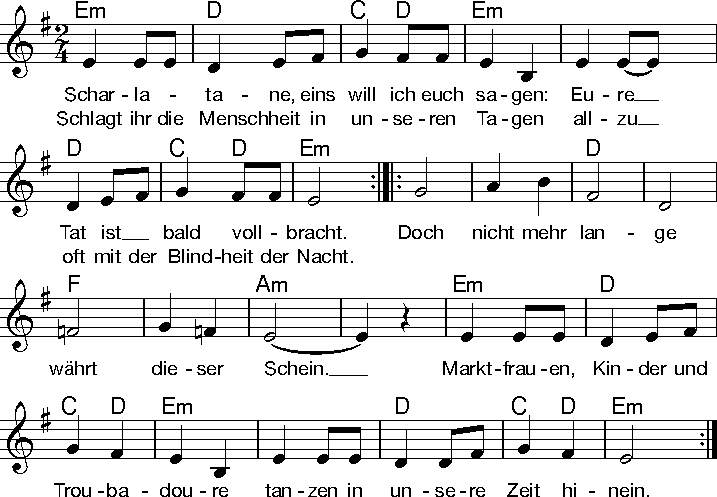
\includegraphics[width=1\textwidth]{Noten/Lied063.pdf}	

\beginverse
\[Em]Sie war’n nicht \[D]lange im \[C]Ne\[D]bel ver\[Em]borgen,
sie hat nicht \[D]lange die \[C]Blind\[D]heit ge\[Em]quält.
\[Em]Sie haben \[D]Einfall um \[C]Ein\[D]fall ge\[Em]boren,
haben \[D]Gefahr und \[C]Frei\[D]heit ge\[Em]wählt.
\lrep Sie sind nicht \[D]feige, \[F]ängstlich und \[Am]klein.
\[Em]Marktfrauen, \[D]Kinder und \[C]Trou\[D]ba\[Em]doure
\[Em]tanzen in \[D]unsere \[C]Zeit \[D]hi\[Em]nein. \rrep
\endverse

\beginverse
^Trotzen der ^Macht, die mit ^Angst ^Menschen ^presste,
die allen ^Mut zu ^fra^gen ver^bannt.
^Feiern in^mitten der ^Ker^ker die ^Feste,
bauen ihr ^Zelt auf ver^bo^tenes ^Land.
\lrep Blumen er^blüh'n im ^grauen Ge^stein.
^Marktfrauen, ^Kinder und ^Trou^ba^doure,
bunter ^Tanz in die ^Welt ^hi^nein. \rrep
\endverse

\endsong

\beginscripture{}
%nix g'fund'n
\endscripture

\begin{intersong}

\end{intersong}